\documentclass[11pt,DIV=10,final]{scrreprt} %11pt legt die generelle Schriftgrösse fest, DIV die Seitenaufteilung (Seitenränder): lieber viele Seiten als zu kleine Seitenränder!
%ändert man "final" zu "draft", werden speicheraufwändige Elemente nicht eingebunden: Genau das richtige für die Plagiatsprüfung

%*************** Paket-Einbindungen: ******************
\usepackage[utf8]{inputenc} %damit man auch Umlaute eingeben kann
\usepackage[bitstream-charter]{mathdesign} % Charter als Standardschriftart
\usepackage[scaled=.82]{DejaVuSansMono} % DejaVuSansMono als Code-Schriftart
\usepackage[T1]{fontenc} %damit Umlaute bei einer pdf-Suche auch erkannt werden
\usepackage{amsfonts,amsmath} %Verwendung von Mathematik-Schriftarten
\usepackage{graphicx} %für Grafiken der Formate jpg, png, pdf
\usepackage{float} % um Abbildung wirklich genau dort zu platzieren
\usepackage{url} %für die gute Darstellung von Internet-Links
\usepackage{hyperref} %für die gute Darstellung von Internet-Links
% \usepackage[ngerman]{babel} %deutsches Sprachpaket
\usepackage[english]{babel} %deutsches Sprachpaket
\usepackage[round]{natbib} %für vereinfachte:wen/Querverweise
\usepackage{listings} % für Quelltext mit Syntax-Highlighting
\usepackage{listings-rust}
\usepackage{hyperref}
\usepackage{svg}
\usepackage{tikz} %für tikz-Grafiken
\usetikzlibrary{graphs} %für Graphen (also auch Neuronale Netze) in tikz

%************** Zusätzliche Einstellungen und eigene Befehle:  **********
\setkomafont{sectioning}{\rmfamily\bfseries\boldmath} % verwende für die Titel die selbe Schriftart wie für Fliesstext

\tikzset{>=stealth} % schönere Pfeilspitzen in TikZ-Grafiken

\lstnewenvironment{cppcode}[1][] % für abgesetzten C++ Code
{\lstset{
	language=C++,
	%backgroundcolor=\color[HTML]{E8F2F2},
	basicstyle=\small\ttfamily,
	keywordstyle=\color{blue},
	commentstyle=\color{brown}, 
	numbers=left,
	%numberstyle=\tiny,
	%frame=leftline,
	%xleftmargin=.04\textwidth,
	inputencoding=utf8,
	extendedchars=true,
	literate={ä}{{\"a}}1 {à}{{\`a}}1 {ö}{{\"o}}1 {ü}{{\"u}}1 {è}{{\`e}}1 {é}{{\'e}}1,
	#1}}{}

\lstnewenvironment{rustcode}[1][] % für abgesetzten rust code
{\lstset{
	language=Rust,
	%backgroundcolor=\color[HTML]{E8F2F2},
	basicstyle=\small\ttfamily,
	keywordstyle=\color{blue},
	commentstyle=\color{brown},
	numbers=left,
	%numberstyle=\tiny,
	%frame=leftline,
	%xleftmargin=.04\textwidth,
	inputencoding=utf8,
	extendedchars=true,
	literate={ä}{{\"a}}1 {à}{{\`a}}1 {ö}{{\"o}}1 {ü}{{\"u}}1 {è}{{\`e}}1 {é}{{\'e}}1,
	#1}}{}
	
\providecommand{\cppinline}{\lstinline[language=C++,basicstyle=\ttfamily,keywordstyle=\color{blue},commentstyle=\color{brown}, literate={ä}{{\"a}}1 {à}{{\`a}}1 {ö}{{\"o}}1 {ü}{{\"u}}1 {è}{{\`e}}1 {é}{{\'e}}1]} % für Inline-C++ Code

\providecommand{\rustinline}{\lstinline[language=Rust,basicstyle=\ttfamily,keywordstyle=\color{blue},commentstyle=\color{brown}, literate={ä}{{\"a}}1 {à}{{\`a}}1 {ö}{{\"o}}1 {ü}{{\"u}}1 {è}{{\`e}}1 {é}{{\'e}}1]} % für Inline-C++ Code

\begin{document}

\begin{titlepage}
\mbox{}\vspace{0.1\textheight}
\begin{center}
\textbf{\Huge Approximating Solutions of the time independent Schrödinger equation}\\[3ex]
Gian Laager\\
\today
\vspace{0.05\textheight}
\begin{center}
	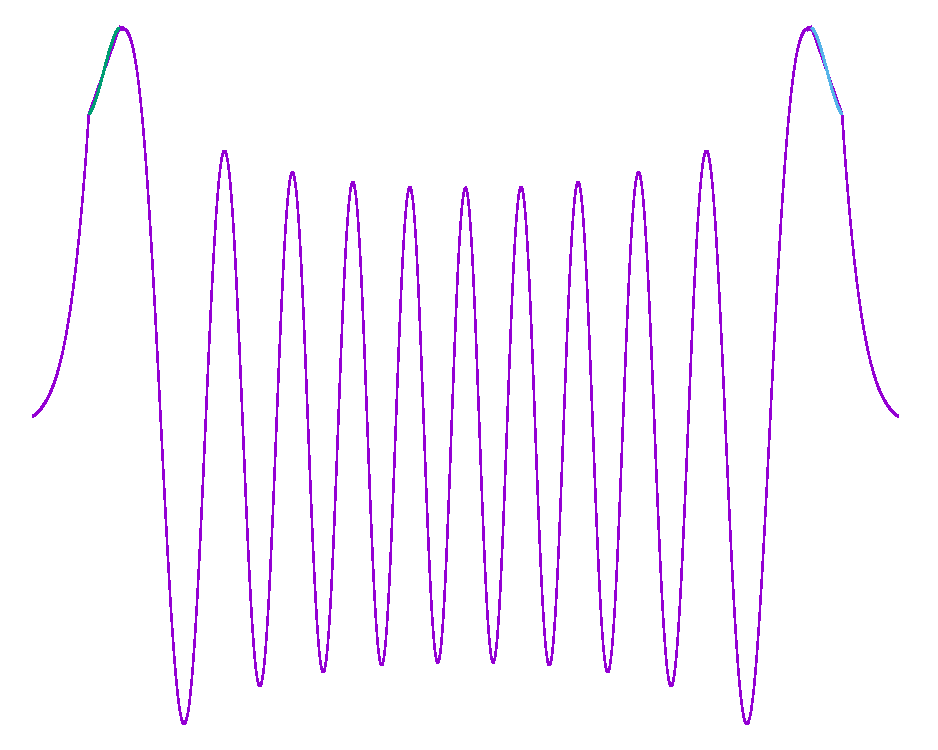
\includegraphics[width=.7\textwidth]{wave_func_square.pdf}
\end{center}
\vspace{0.05\textheight}
Maturaarbeit\\
Kantonsschule Glarus\\
Betreuer: Linus Romer\\
Referent: Beat Temperli
\end{center}
\end{titlepage}

\pagenumbering{roman}   % i, ii, iii, iv, ...

\tableofcontents %Inhaltsverzeichnis

\chapter{Introduction}\pagenumbering{arabic}  % 1, 2, 3, 4, ...
\section{Schrödinger Equation}
In 1926 Erwin Schrödinger changed our understanding of quantum physics with the Schrödinger equation. Based on the observations of de Broglie that particles
behave like waves he developed a wave equation which describes how the waves move and change in a given potential $V(x)$ or Hamiltonian $\hat{H}$.
\begin{center}
\begin{math}
  i\hbar {\frac {\partial }{\partial t}}\Psi (x,t)=\left[-{\frac {\hbar ^{2}}{2m}}{\frac {\partial ^{2}}{\partial x^{2}}}+V(x,t)\right]\Psi (x,t)
\end{math}
\end{center}
Or more general
\begin{center}
\begin{math}
  i\hbar {\frac {\partial }{\partial t}}\Psi (x,t)=\hat{H} \Psi(x,t)
\end{math}
\end{center}

The time independent version that is going to be used later, it ignores the change over time and is much simpler to solve since it is \emph{\textbf{only}} an ODE instead of a PDE.
\begin{center}
\begin{math}
  E \psi (x)=\hat{H} \psi(x)
\end{math}
\end{center}
or
\begin{center}
\begin{math}
  -{\hbar^{2} \over 2m}  {d^{2} \psi \over dx^{2}} (x) + V(x) \psi(x) = E \psi(x)
\end{math}
\end{center}

Even with the time independent equation it is very difficult to get analytical solutions, because of this there are mainly three approaches to
approximate solutions of $\psi(x)$, perturbation theory, density functional field theory and WKB approximation. Perturbation theory's goal is to give an analytical approximation which means it
is extremely difficult to implement it for a computer. WKB on the other hand is much better since it is to some degree a step by step manual.
\section{Rust}
Rust is one of the newer programming languages and attempts to replace C/C++ which are notoriously difficult to work with. It supports both functional and object-oriented para dimes. It is much safer in terms of memory and promises the same performance as C. One of the goals of Rust is fearless concurrency which means everybody should
be able to write concurrent code without deadlocks and data races. This means calculations can utilize the full potential of the CPU without countless hours of debugging.

Personally I like programming languages that support functional para dimes when I'm programming something that uses a lot of math since functional programming languages are designed according to mathematical concepts that also govern the problem. This usually results in rather neat solutions.

Rust as of the time of writing this document is not yet standardized meaning the code provided might no longer be correct with one of the newer Rust versions.

\chapter{Methods}
\section{Approximation Scheme}
\label{meth:wkb:approximation-scheme}
There are mainly three approximation methods used to solve for the actual wave function itself. There is perturbation theory which breaks the problem down in to ever smaller sub-problems that then can be
solved exactly. This can be achieved by adding something to the Hamiltonian operator $\hat{H}$ which can then be solved exactly. But \textit{perturbation theory is inefficient compared to other approximation
methods when calculated on a computer} \citep[Introduction]{van2014density}.

The second is Density functional field theory, it has evolved over the years and is used heavily in chemistry to calculate properties of molecules and is also applicable for the time dependent Schrödinger
equation. It is something that might be interesting to add to the program in the future.
\\

The program uses the third method WKB approximation, it is applicable to a wide verity of linear differential equations and works very well in the case of the Schrödinger equation.
Originally it was developed by Wentzel, Kramers and Brillouin in 1926. It gives an approximation to the eigenfunctions of the Hamiltonian $\hat{H}$ in one dimension. The approximation is best
understood as applying to a fixed range of energies as $\hbar$ tends to zero \citep[p.~305]{hall2013quantum}. This is not a physically correct explanation because one can not assume that $\hbar$ is small since it has units, but there is another interpretation that is physically more valid that will be discussed in section~\ref{meth:wkb:valid}.

\subsection{Example}
This example is from~\cite[An example]{wiki:wkb}.

Lets solve the ordinary differential equation
\[
  \epsilon^{2} {d^{2}y \over dx^{2}} = Q(x)y
\]
where $Q(x)$ is an arbitrary function that is not $Q(x) = 0$ and $\epsilon$ is small. Note that this example relates to the Schrödinger equation
where $\epsilon = -{\hbar^{2} \over 2m}$ and $Q(x) = E - V(x)$.

Replace $y$ with
\[
  y(x) = exp({1 \over \delta} \sum_{n=0}^{\infty}{\delta^{n}S_{n}(x)})
\]
resulting in the equation
\begin{equation}
\label{eq:wkbexpand}
  \epsilon^{2}{1 \over \delta^{2}}(\sum_{n=0}^{\infty}{\delta^{n}S'_{n}(x)} + {1 \over \delta}(\sum_{n=0}^{\infty}{\delta^{n}S''_{n}(x)})) = Q(x)
\end{equation}
As an approximation set the upper bound of the sum to be $2$ instead of $\infty$, then~\ref{eq:wkbexpand} can be written as
\begin{equation}
\label{eq:wkbapprox}
 \frac{\epsilon^2}{\delta^2}S_0'^2 + \frac{2\epsilon^2}{\delta}S_0'S_1' + \frac{\epsilon^2}{\delta}S_0'' = Q(x)
\end{equation}
If we go further and solve for $S_{0}$ and $S_{1}$ we will get that
\begin{align}
	S_0(x) = \pm \int_{x_0}^x \sqrt{Q(t)}\,dt \\
	S_1(x) = -\frac{1}{4}\ln Q(x) + k_1
\end{align}
this means that our approximate solution of $y$ is
\[
y(x)\approx c_{1}Q^{-{\frac {1}{4}}}(x)\exp \left[{\frac {1}{\epsilon }}\int _{x_{0}}^{x}{\sqrt {Q(t)}}\,dt\right]+c_{2}Q^{-{\frac {1}{4}}}(x)\exp \left[-{\frac {1}{\epsilon }}\int _{x_{0}}^{x}{\sqrt {Q(t)}}\,dt\right]
\]
here $c_{1}$, $c_{2}$ depend on the boundary conditions and can also be used to renormalize the function. $x_{0}$ will later be discussed in section~\textit{\textbf{(...)}}. It is important to have the right value for $x_{0}$ which depends on $V(x)$ and $E$ although I have not yet manged to find out the connection.

\subsection{Validity}
\label{meth:wkb:valid}
\textit{\textbf{Dieser abschnitt ist momentan nur fürs Probe Kapitel muss ich noch besser nach Rechnen und genau verstehen}}

The approximation that was made in equation~\ref{eq:wkbexpand} to~\ref{eq:wkbapprox} that we ignored the terms of $n > 2$ and assumed that they are small.
\[
\epsilon \left|{\frac {dQ}{dx}}\right|\ll Q(x)^{2}
\]

Without the assumption that $\hbar$ is infact \textit{small} the equation can also be interpreted such that the potential $V(x)$ has to vary slowly compared to $(V(x) - E)^{2}$.

During calculations I noticed that it is crucial what values $x_{0}$ has sinse some times the results can not be valid.

\section{Newtons Method}
Newton's method, also called the Newton-Raphson method, is a root-finding algorithm that uses the first few terms of the Taylor series of a function $f(x)$ in the vicinity of a suspected root
\citep{math:newton}. It makes a sequence of approximations of a root $x_{n}$ that in sure tent cases converges to the exact value where
\[
  \lim _{n \to \infty}f(x_{n}) = 0
\]

The sequence is defined as
\begin{align*}
  x_{0}=a \\*
  x_{n+1}=x_{n}-{f(x_{n}) \over f'(x_{n})}
\end{align*}

Visually this looks like figure~\ref{fig:newton-ilust} $f(x) = (x-1)(x+1)(x-2)$.
\begin{figure}
	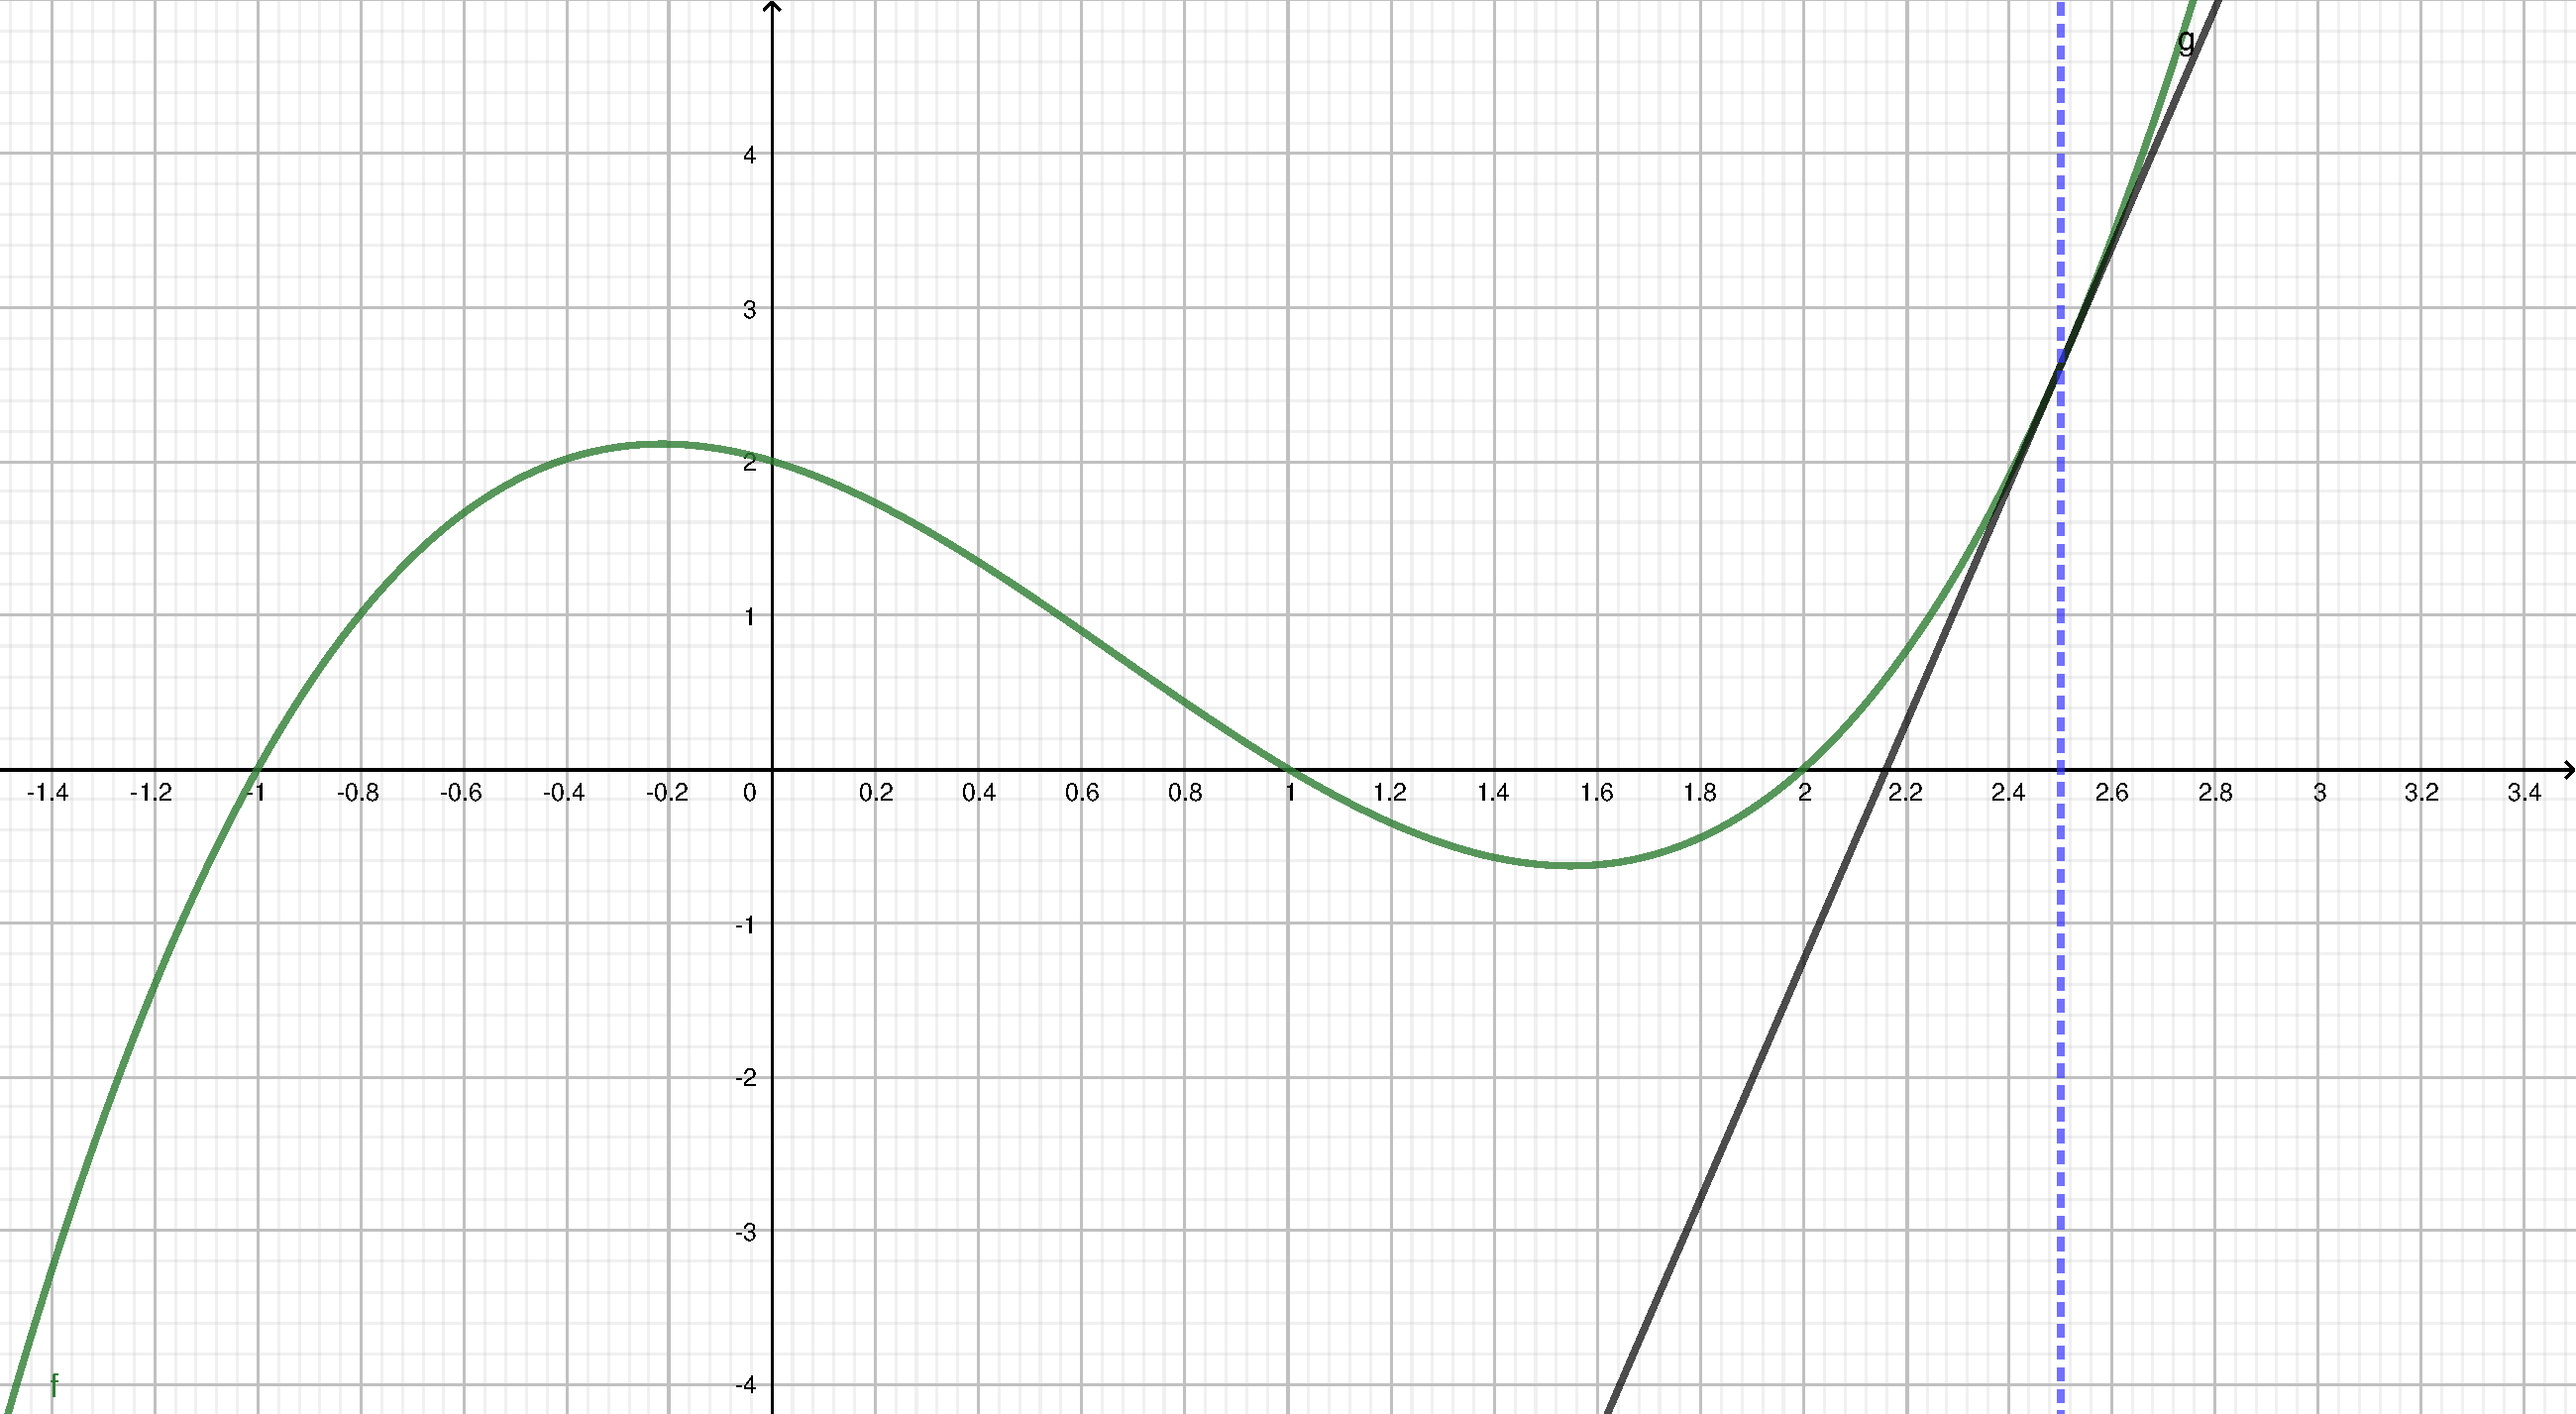
\includegraphics[width=\textwidth]{newtons-method.pdf}
	\caption{Illustration of Newtons method, $f(x) = (x-1)(x+1)(x-2)$.}
	\label{fig:newton-ilust}
\end{figure}
The blue line indicates the initial guess which in this case is $2.5$ the black line ($g(x)$) is a tangent to $f(x)$ at $(guess, f(guess))$ the next guess will be where
the tangent intersects the x-Axis (solution of $g(x) = 0$). This will converge rather quickly compared to other methods such as Regula-Falsi.

\pagebreak
\begin{rustcode}\nopagebreak
pub fn newtons_method<F>(f: &F, mut guess: f64, precision: f64) -> f64
    where
        F: Fn(f64) -> f64,
{
    loop {
        let step = f(guess) / derivative(f, guess);
        if step.abs() < precision {
            return guess;
        } else {
            guess -= step;
        }
    }
}
\end{rustcode}

In rust the sequence is implemented with a function that takes a closure \rustinline{f}, the initial guess \rustinline{guess} and a stop condition \rustinline{precision} the function will return if
$|{f(x_{n}) \over f'(x_{n})}|$ is less than \rustinline{precision}.

From the structure of the algorithm it is very tempting to implement it recursively, but by using a loop it is much faster since there are no unnecessary jumps and the precision can (at least in theory) be $0$ without causing a stack overflow.

\section{Derivatives}
The precision gained by calculating derivatives analytically would come with a massive overhead both in development and in performance, one would have to implement all the rules of differentiation and create some representation of an actual function to which those rules could be applied. I wrote an implementation of this in Go and not much accuracy can actually be gained.

A much easier approach is to approximate it. The definition of a derivative of a function $f(x)$ is
\[
  {df \over dx} = \lim_{h \to 0}{f(x + h) - f(x) \over h}
\]
The limit can very easily be approximated with
\[
  {f(x + \frac{\delta}{2}) - f(x - \frac{\delta}{2}) \over \delta}
\]
were $\delta$ needs to be small yet not so small that it exceeds the 16 digit precision of double. I chose $\delta = \sqrt{2^{-52}}$, because $\epsilon = 2^{-52}$ is the smallest double precision floating point number where
$1 + \epsilon \ne 1$. The square root ensures that still enough precision remains. After some further research the function should be implemented the same way as described by Boost~(C++~library).

\pagebreak
\begin{rustcode}
pub fn derivative<F, R>(f: &F, x: f64) -> R
    where
        F: Fn(f64) -> R,
        R: Sub<R, Output=R> + Div<f64, Output=R>,
{
    let epsilon = f64::epsilon().sqrt();
    (f(x + epsilon / 2.0) - f(x - epsilon / 2.0)) / epsilon
}
\end{rustcode}

\rustinline{f64::epsilon()} this is the difference between `1.0` and the next larger representable number~\citep{rust:f64:epsilon}. \rustinline{derivative} is implemented not only for \rustinline{f64} but for all types that support subtraction and division by \rustinline{f64} this means it can also be used for closures with real inputs and complex outputs.

\section{Integration}
The same principles apply to integrals as to derivative it would not be a great benefit to implement an analytic integration system. Integrals would also be much more difficult to implement than
derivatives since integrals can not be broken down in to many smaller integrals that can be computed easily instead it needs to be solved as is.

One approach would be to use the same method as with the derivative, take the definition with the limit and use a small value but this method can be improved in this case, since integrals calculate
areas under curves a trapeze is more efficient and accurate then the rectangle that results from the definition.

\begin{figure}[h]
  \centering
	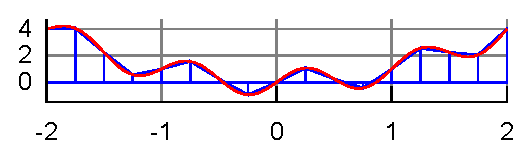
\includegraphics[width=0.7\textwidth]{Integration_trapezoid.pdf}
	\caption{Illustration of integration with trapeze from \cite{wiki:integration-methods}.}
	\label{fig:integration-ilust}
\end{figure}

Figure \ref{fig:integration-ilust} shows visually how the methods work, each blue trapeze from start ($a$) to end ($b$) has an area of
\[
\int _{a}^{b}f(x)\,dx\approx (b-a)f\left({\frac {a+b}{2}}\right).
\]
One trapeze would be fairly inaccurate to calculate the area under the function but as the area from $a$ to $b$ is subdivided further the result become better and better.

The general structure of the algorithm can very easily be run in parallel since it doesn't matter in which order the segments are added together and the segments also don't dependent on one another.
In rust this is implemented using rayon. Rayon is an implementation for parallel iterators meaning that normal data structures that implement \rustinline{std::iter} can be run in parallel \emph{just} by
changing \rustinline{::iter()} to \rustinline{::par_iter()}. This might not work in all cases because of memory safety but in this case the borrow checker will throw an error and the code wont compile.

\begin{rustcode}
pub trait ReToC: Sync {
    fn eval(&self, x: &f64) -> Complex64;
}

pub struct Point {
    pub x: f64,
    pub y: Complex64,
}
\end{rustcode}
These functions were implemented very early and need some refractory. Such that functions with states, like wave functions that store parameters, can be integrated there is a trait
\rustinline{ReToC}. \rustinline{ReToC} describes a function $f: \mathbb{R} \to \mathbb{C}$ (\rustinline{Fn(f64) -> Complex64}).

\rustinline{Point} stores both the input (x) and the output (y) of a function.

\begin{rustcode}
pub fn evaluate_function_between(f: &dyn ReToC, a: f64, b: f64, n: usize) -> Vec<Point> {
    if a == b {
        return vec![];
    }

    (0..n)
        .into_par_iter()
        .map(|i| index_to_range(i as f64, 0.0, n as f64 - 1.0, a, b))
        .map(|x| Point { x, y: f.eval(&x) })
        .collect()
}
\end{rustcode}
\rustinline{ReToC} can be passed to \rustinline{evaluate_function_between}
it calculates \rustinline{n} points between an interval from \rustinline{a} to \rustinline{b} and returns a vector of \rustinline{Point}.

\pagebreak
\begin{rustcode}
pub fn trapezoidal_approx(start: &Point, end: &Point) -> Complex64 {
    return complex(end.x - start.x, 0.0) * (start.y + end.y) / complex(2.0, 0.0);
}

pub fn index_to_range(x: f64, in_min: f64, in_max: f64, out_min: f64, out_max: f64) -> f64 {
    return (x - in_min) * (out_max - out_min) / (in_max - in_min) + out_min;
}

pub fn integrate(points: Vec<Point>, batch_size: usize) -> Complex64 {
    if points.len() < 2 {
        return complex(0.0, 0.0);
    }

    let batches: Vec<&[Point]> = points.chunks(batch_size).collect();

    let parallel: Complex64 = batches
        .par_iter()
        .map(|batch| {
            let mut sum = complex(0.0, 0.0);
            for i in 0..(batch.len() - 1) {
                sum += trapezoidal_approx(&batch[i], &batch[i + 1]);
            }
            return sum;
        })
        .sum();

    let mut rest = complex(0.0, 0.0);

    for i in 0..batches.len() - 1 {
        rest += trapezoidal_approx(&batches[i][batches[i].len() - 1], &batches[i + 1][0]);
    }

    return parallel + rest;
}
\end{rustcode}
The actual integration happens in \rustinline{integrate}, it calculates the areas of the trapezes between the points passed to it. For optimization 1000 trapezes are calculated per thread because it would
take more time to create a new thread then to actually do the calculation, this has to be further investigated and 1000 might not be optimal. The calculations performed per thread are called a batch,
after all batches have been calculated the boundaries between batches also has to be considered therefor they are added in the end with \rustinline{rest}

%
\begin{appendix} %Anhang falls nötig
%
\chapter{Source Code}
At the moment the code is only available on \url{https://github.com/Gian-Laager/Schroedinger-Approximation}

\chapter{Detailed Calculations}
% TODO
\end{appendix}
\chapter*{Bildquellen}
%
Wo nicht anders angegeben, sind die Bilder aus dieser Arbeit selbst erstellt worden. Das Titelbild stammt aus.
%
\bibliographystyle{plainnatromer}
\bibliography{marbeit}

%
\chapter*{Selbständigkeitserklärung}
%
Hiermit bestätige ich, Gian Laager, meine Maturaarbeit selbständig verfasst und alle Quellen angegeben zu haben.\\\newline
Ich nehme zur Kenntnis, dass meine Arbeit zur Überprüfung der korrekten und vollständigen Angabe der Quellen mit Hilfe einer Software (Plagiaterkennungstool) geprüft wird. Zu meinem eigenen Schutz wird die Software auch dazu verwendet, später eingereichte Arbeiten mit meiner Arbeit elektronisch zu vergleichen und damit Abschriften und eine Verletzung meines Urheberrechts zu verhindern. Falls Verdacht besteht, dass mein Urheberrecht verletzt wurde, erkläre ich mich damit einverstanden, dass die Schulleitung meine Arbeit zu Prüfzwecken herausgibt.\\\newline
Ort\hspace{4cm} Datum\hspace{4cm}  Unterschrift
%
\end{document}
